\documentclass{article}
\usepackage[T1]{fontenc}
\usepackage{lmodern}
\usepackage{graphicx}
\usepackage{amsmath,amssymb}
\usepackage[a4paper,margin=2cm]{geometry}
\usepackage[absolute,overlay]{textpos}
\setlength{\TPHorizModule}{1mm}
\setlength{\TPVertModule}{1mm}
\usepackage[indonesian]{babel}
\usepackage{hyperref}
\setlength{\emergencystretch}{2em}
% unit: Halaman 8

\begin{document}

% === Halaman 8 (python/native) ===

8

• Enkripsi dan dekripsi Caesar Cipher dapat dilakukan secara matematis

• Misalkan setiap huruf alfabet dikodekan ke dalam integer dari 0 sampai 25 sebagai 

berikut:







  maka, secara matematis Caesar Cipher dirumuskan sebagai:

 Enkripsi: c = E(p) = (p + 3) mod 26

 Dekripsi: p = D(c) = (c – 3) mod 26

Ket:   p = plainteks;   c = cipherteks

% deskripsi: gambar native xref 66
\noindent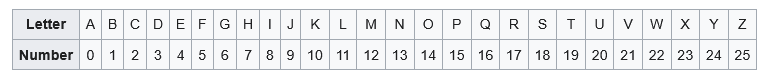
\includegraphics[width=0.85\textwidth]{../../images/python/page_008_img_01.png}

\end{document}
